\documentclass{article}

\usepackage[utf8]{inputenc}
\usepackage{graphicx}
\usepackage{float}
\usepackage{tikz}
\usepackage{amsmath}
\usepackage{graphicx,lipsum,afterpage,subcaption}
\usepackage{enumitem}
\usepackage{hyperref}
\usepackage{imakeidx}
\makeindex
\renewcommand{\listfigurename}{Figures}

\title{\textbf{Software Requirements Specification}}
\begin{document}

\begin{figure}
    \centering
    
\includegraphics[height=5cm,width=5cm]{pitt-min.jpg}
\end{figure}

\author{Thomas Bui, Justin Carter, Patrick Flaherty, Wesley Miller, Philip Seitz}

\date{}



\maketitle

\newenvironment{subs}
  {\adjustwidth{3em}{0pt}}
  {\endadjustwidth}

\pagebreak 


\begin{center}
\Title{}
Change Log
\newline
 \begin{tabular}{||c c c c||} 
 \hline
 Version Number & Date & Description of the Change & Team Member \\ [0.5ex] 
 \hline\hline
 1 & October 3, 2019 & Initial Version & All Members \\ 
 \hline
  &  &  &  \\
 \hline
  &  &  &  \\
 \hline
  & &  &  \\
 \hline
  &  &  &  \\ [1ex] 
 \hline
\end{tabular}
\end{center}


\pagebreak
\newpage
\tableofcontents
\newpage

\section{Introduction}
\paragraph{}
This section of the Software Requirements Specification (SRS \index{SRS}) document provides the purpose of the SRS\index{SRS}, scope of the SRS\index{SRS}, acronyms and abbreviations used in the SRS\index{SRS}, list of references, and an overview of the SRS\index{SRS} document’s structure.

    
    \subsection{Purpose}
    \paragraph{}
    The purpose of this project is to develop a fully operational demonstration of the control center, communications, train, and track control system with simulator for the transit system for review by the Port Authority of Allegheny County (PAAC) procurement committee. The intended use for this project will be for the North Shore Extension of the Light Rail Transit system.

    
    \subsection{Scope}
    \paragraph{}
     The purpose of this project is to design and implement a new Centralized Traffic Control Center and Signaling System for Light Rail Transit system. The final system will be an executable that will demonstrate a fully operational control center, communications, train and track control system simulator for the transit system. This system would include a specification and implementation of a Centralized Traffic Control Center, a Track Controller\index{Track Controller}, a Track Model\index{Track Model}, a Train Controller\index{Train Controller}, and a Train Model\index{Train Model}. These modules would all be interface-able with a user. Above all, we hope to provide a comfortable user experience along with the best pricing available. 

    
    \subsection{Definitions, Acronyms, and Abbreviations}
    \paragraph{} The following are a list of terms, each followed by synonyms and abbreviations. A definition of each of the terms then follows:
    \begin{itemize}
        \item Train Control Signaling System - TCSS\index{TCSS}
            \begin{itemize}
            \item The Train Signaling System is the complete deliverable which this SRS \index{SRS} shall specify.
            \end{itemize}
        \item Centralized Traffic Control - CTC \index{CTC}
            \begin{itemize}
            \item The Central Office is one of the major modules of the TCSS\index{TCSS}. The CTC \index{CTC} is able to track the locations of the trains in the railway, as well as communicate to these trains important and vital information.
            \end{itemize}
        \item Operation Control Center - OCC
            \begin{itemize}
            \item See \emph{Centralized Traffic Control}
            \end{itemize}
        \item Central Office
            \begin{itemize}
            \item See \emph{Centralized Traffic Control}
            \end{itemize}

        \item Track Controller \index{Track Controller}
            \begin{itemize}
            \item This is a major module of the TCSS\index{TCSS}. The Track Controller \index{Track Controller} is responsible for sending important information to both the CTC \index{CTC} and the Train Controller \index{Train Controller} (Through the Track and Train Models\index{Train Model}). It also is responsible for controlling the state of the tracks, such as track switching and railway crossing. This runs a PLC \index{PLC} and is configurable on a per-Track Controller \index{Track Controller} basis.
            \end{itemize}
        \item Train Controller \index{Train Controller}
            \begin{itemize}
            \item This is a vital  \emph{(See Vital)} component of the TCSS\index{TCSS}. It is responsible for regulating the speed of the train. It is also responsible for controlling various other features of the Train Model\index{Train Model}. It is directly interface-able by the train driver, and will be capable of being controlled in both automatic and manual modes. 
            \end{itemize}
        \item Track Model \index{Track Model}
            \begin{itemize}
            \item This is a major component of the TCSS\index{TCSS}. It is a digital representation of the track with which the Train Model\index{Train Model} rides over, and the model which the Track Controller \index{Track Controller} is responsible for. This is configurable via a formatted csv file that will allow the user to simulate and control over any track diagram.
            \end{itemize}
        \item Train Model\index{Train Model}
            \begin{itemize}
            \item This is a major component of the TCSS\index{TCSS}. It is a digital representation of the Train with which the Train Controller \index{Train Controller} is responsible for. Furthermore it is a representation of the effect of Newtonian physics on the TCSS\index{TCSS} decision making.
            \end{itemize}
        \item Port Authority of Allegheny County - PAAC
            \begin{itemize}
            \item A public transit agency within Pennsylvania.
            \end{itemize}    
        \item Programmable Logic Controller - PLC \index{PLC}
            \begin{itemize}
            \item This is a logic controller that is specially programmable on a per-device basis. It is often adapted for the control of systems and devices that require a high reliability and ease of programming.
            \end{itemize}
        \item Vital
            \begin{itemize}
            \item Safety-Critical
            \end{itemize}
        \item Java Runtime Environment - JRE
            \begin{itemize}
            \item  The JRE is a virtual machine that enables a host computer to execute programs written in Java.
            \end{itemize}
        \item Office Open XML Workbook - XLSX
            \begin{itemize}
            \item  Office Open XML is a zipped, XML-based file format developed by Microsoft for representing spreadsheets, charts, presentations and word processing documents.
            \end{itemize}
        \item Graphic User Interface\index{interface} - GUI
            \begin{itemize}
                \item An electronic user interface \index{interface} displayed through a screen so that a user may interact with software.
            \end{itemize}
    \end{itemize}
    
    \subsection{References}
     \begin{itemize}
        \item Blackpool Flexity Tram Specifications, Bombardier Inc., 2009. Contained in professor-supplied Project Information directory.
    \end{itemize}

    \subsection{Overview}
    The following sections of this document go into more of the details of the TCSS\index{TCSS}. Section 2 is customer/user focused, discussing the system's interfaces\index{interface}, and requirements for the computer running the program. Section 3 will be of more interest to developers; it outlines requirements that must be met, both functional and structural, in order to consider the system satisfactorily operational. Sections 4 and 5 are more administrative in nature, outlining the process by which future changes to this document and the overall system must be approved. Section 6 includes a list of figures and an index.

    
\section{Overall Description}
\paragraph{}
The TCSS\index{TCSS} is a software program, comprised of multiple modules, that will be capable of controlling and simulating a train transit system. The several modules will be used by different types of users, such as Train Drivers, Track Builders\index{Track Builder}, and Transit Dispatchers\index{Dispatcher}. The system must be capable of operating safely and the simulator must be capable of running for at least a minimum of 24 hours without fail or stop. The client shall be capable of installing a new track layout and the software must be capable of adapting to this new track layout. The specifics of this product are described within this section.
    
    \subsection{Product Perspective}
    \paragraph{}
    
    The TCSS\index{TCSS} shall interface \index{interface} with multiple different portions of an already present light rail system. 
    
    \begin{itemize}
        \item The Track Controller \index{Track Controller} will be installed to Wayside Controllers throughout the existing railway.
        \item The Track Model \index{Track Model} will be specified according to the existing track, beacons, stations, and crossings.
        \item The Train Model\index{Train Model} will be specified according to the physical requirements of the existing rail system's tram. See references(1).
        \item The Train Controller \index{Train Controller} will be installed within the existing rail system's tram.
    \end{itemize}
    
    \paragraph{}
    Additionally, the TCSS,\index{TCSS} CTC \index{CTC} and Simulator modules will be installed within an personal computer running Windows 10. 
    
    \begin{figure} [!h]
    \centering
    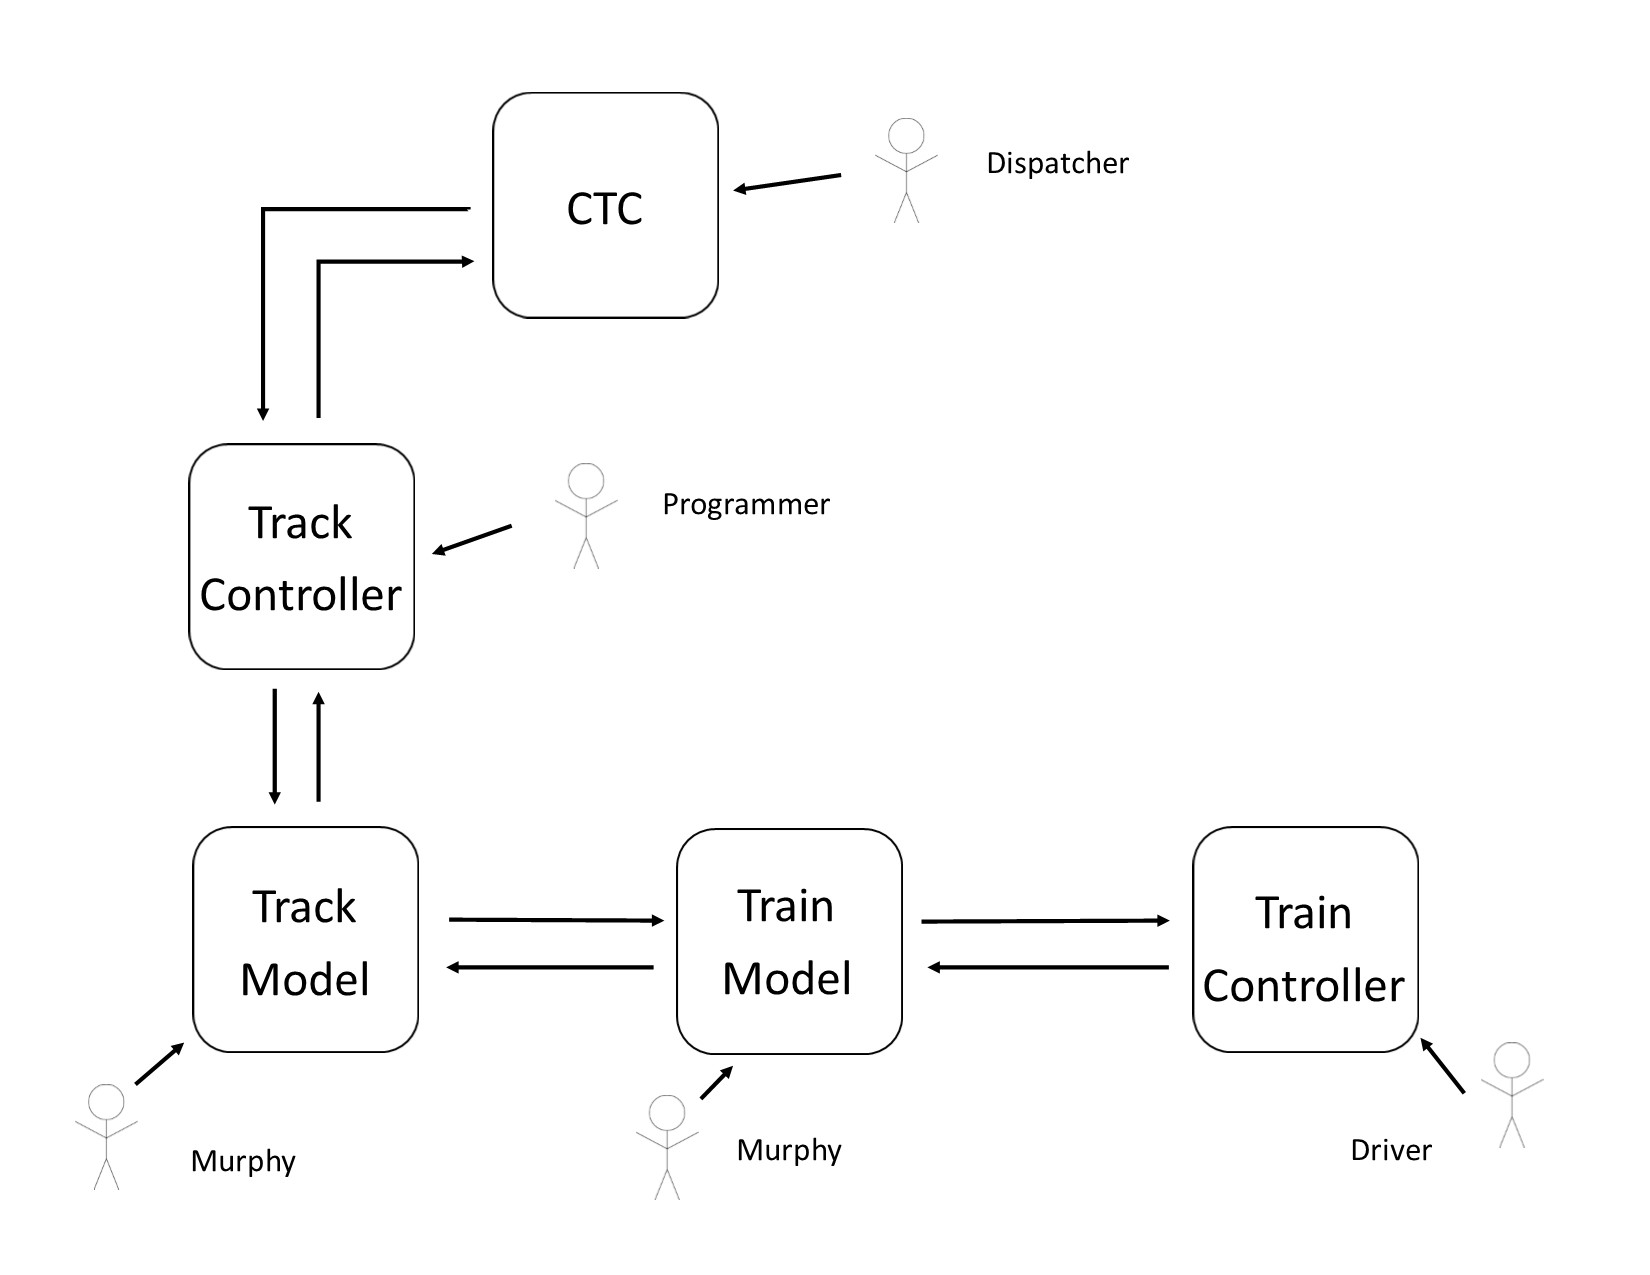
\includegraphics[height=9cm,width=13cm]{SystemBlockDiagram.jpg}
    \caption{Block Diagram of TCSS\index{TCSS}}
    \end{figure}
    
    \paragraph{}
    The following subsections describe how the software operates inside various constraints.

    \subsubsection{System Interfaces\index{interface}}
    \paragraph{}
    
    
    \begin{itemize}
        \item The PLC \index{PLC} must be compatible with the Wayside Controllers of the existing Transit System. In order to accommodate this, the PLC \index{PLC} shall be written in one of the following formats:
        \begin{itemize}
            \item Ladder Diagram 
            \item Functional Block Diagram
            \item Structured Text
            \item Instruction List
            \item Sequential Function Charts
            \item Specially Developed Boolean Based Language
        \end{itemize}
    \item The CTC \index{CTC} must be compatible with the existing format of train schedules. In order to accommodate this, the user shall upload a schedule file, in the form of a xlsx, which will then be parsed for known station names and time requirements. \emph{See 3.1 External Interfaces\index{interface}.} 
    \item The Track Model \index{Track Model} module must be compatible with the specifications of the existing track layout. The user shall upload a track layout file, in the form a xlsx, which will then be parsed for block properties, station locations, switch locations, speed limit, railroad crossings. \emph{See 3.1 External Interfaces.}
    \item The TCSS\index{TCSS} shall utilize and interface \index{interface} with the Java Runtime Environment.
    \end{itemize}

    \subsubsection{Interfaces\index{interface}}
    \begin{itemize}
        \item The CTC \index{CTC} shall contain a GUI through which the Dispatcher \index{Dispatcher} will be able to view the current state of the railway system.  There the Dispatcher \index{Dispatcher} can view all of the information about track blocks and active trains in the system and can also dispatch new trains to a location.  Additionally the Dispatcher \index{Dispatcher} shall be capable of closing and opening specific blocks of the track for maintenance. 
        
        \item The Train Controller \index{Train Controller} module shall contain a GUI through which the Train Driver will be capable of controlling various aspects of the train's operation, as well as observe other characteristics of the controller's behavior. Additionally, the Train Controller \index{Train Controller} shall be installed on a per tram basis so that a Train Engineer \index{Train Engineer} shall specify individual characteristics of the Train Controller\index{Train Controller}.
        
        \item The Track Controller \index{Track Controller} module shall contain a GUI where the track engineer shall upload a PLC \index{PLC} file containing Boolean logic to each Track Controller \index{Track Controller}. After upload, the track engineer shall see all outputs of the Track Controller \index{Track Controller} GUI.
        
        \item The Track Model \index{Track Model} shall contain a GUI through which the Track Builder \index{Track Builder} will be able to upload a desired track layout file, which the TCSS\index{TCSS} will use to initialize the track. After the setup, the Track Model \index{Track Model} will include a GUI that allows a user to observe the current status of all components of the track architecture for the purposes of validation. This includes failure status of track blocks, static information in beacons, locations and orientations of track switches, locations of railroad crossings, train locations, and locations of stations.
        
        \item The Train Model\index{Train Model} shall contain a GUI through which the behavior of a train can be emulated for purposes of validation. It shall also interface \index{interface} directly with other modules to simulate the physical behavior of a real train.
    \end{itemize}

    \subsubsection{Hardware Interfaces}
    \paragraph{}
    The system has no hardware interface \index{interface} requirements.

    \subsubsection{Software Interfaces}
    \begin{itemize}
        \item Windows Operating System\textregistered\; by Microsoft\textregistered, version 10, from Microsoft\textregistered
        \begin{itemize}
            \item The host system of the TCSS\index{TCSS} must operate within a Windows operating system for the purpose of file navigation and management.
        \end{itemize}
        \item Java\texttrademark \;Runtime Environment (JRE) by Oracle\textregistered, version 8, from Oracle\textregistered.
        \begin{itemize}
            \item The host system of the TCSS\index{TCSS} must have the specified installation of the JRE to execute the program.
        \end{itemize}
    \end{itemize}
    
    \subsubsection{Communications Interfaces}
    \paragraph{}
    There are no communication interface\index{interface}s or protocols for this system.

    \subsubsection{Memory Constraints}
    \paragraph{}
    The program is required to run on a Microsoft Surface Pro Tablet, therefore it must not exceed 8GB of RAM. Additionally, the implementation of the TCSS\index{TCSS} shall utilize as little memory as possible to minimize resource consumption on the host system.

    \subsubsection{Operations}
    \paragraph{}
    No business operations affect the design of the TCSS\index{TCSS}.
    

    \subsubsection{Site Adaptation Requirements}
    \paragraph{}
    \begin{itemize}
        \item The user can enter Error Simulation mode from the menu screen to access a simulation of the train system where the user can manipulate the system to check failure methods.
        \item In order to run the program correctly, a track layout excel file (.xlsx) shall be uploaded to the system to produce the track diagram. 
        \item Should the automatic scheduler be used, a schedule excel file (.xlsx) shall be uploaded to the system for reference.
        \item The PLC \index{PLC} files shall be imported on a per-Track Controller \index{Track Controller} basis.
    \end{itemize}
    
    \paragraph{}
    No modification of the user's host system shall be necessary as long as it satisfies the requirements listed within this document.
    
    \subsection{Product Functions}
    \paragraph{}
    The product will provide functions for scheduling, dispatching, monitoring, and tracking trains. Users shall be able to input a track layout and input schedules into the program to simulate a route. The program will notify the users of emergencies and failures and ensure the safety of the passengers on-board. 

    \subsection{User Characteristics}
     \begin{itemize}
         \item 
         The Dispatcher\index{Dispatcher} – This user oversees the CTC\index{CTC}. They need to be able to understand the UI in the system so that they may safely dispatch trains and oversee the system. Additionally, they shall be able to close and open portions of the track.
         \item
         The Train Driver – This user is on the train itself and shall be capable of manipulating the state of the train in case of emergencies.
        \item
         The Train Engineer\index{Train Engineer} – This user is responsible for installing and adjusting the kinetic motion constants of the Train Controller\index{Train Controller}.
         \item
         The Passenger – This user is anybody riding the trains of the TCSS\index{TCSS}, and is capable of manipulating the system via the Train Model\index{Train Model}'s emergency brake.
         \item
         The Track Engineer – This user is responsible for manipulating the wayside controller. This user imports the PLC \index{PLC} program.
         \item
         The Track Builder\index{Track Builder} – This user is responsible for designing and importing the track layout for the Track Model\index{Track Model}. 
         \item
         The Validation Engineer – This user is in charge of causing errors to verify that the system works correctly.
     \end{itemize}
     
    \subsection{Constraints}
    \begin{itemize}
        \item The system shall be easily understood by the user.
        \item The system shall be written in Java.
        \item All sub-modules shall integrate with each other. 
        \item The sub-modules shall all contain their own GUI.
        \item The system shall operate reliably in the environment in which it is operating.
        \item The system shall be safety critical. In particular the Train Controller \index{Train Controller} and Track Controller \index{Track Controller} shall be vital.
        \item The Train Controller \index{Train Controller} module is only capable of communicating with the Train Model\index{Train Model}
        \item The Train Model\index{Train Model} module is only capable of communicating with the Train Controller \index{Train Controller} and Track Model\index{Track Model}.
        \item The Track Model \index{Track Model} module is only capable of communicating with the Track Controller \index{Track Controller} and the Train Model\index{Train Model}.
        \item The Track Control module is only capable of communicating with the Track Model \index{Track Model} and the CTC\index{CTC}.
        \item The CTC \index{CTC} module is only capable of communicating with the Track Controller \index{Track Controller}
        \item The beacons shall contain a static 128 characters of information, this can not be changed during run-time of the system or simulation.
        \item The track shall not be reconfigured during run-time. Neither shall the PLC\index{PLC}s be manipulated during run-time.
        \item The Train Model\index{Train Model} will only operate at the constraints required in the Blackpool Flexity tram specifications document. \emph{See 1.4 References}
        \item The track circuit shall pass information with no time or bandwidth constraints. However, the track circuit shall only be used to send the speed limit and authority to the Train Model\index{Train Model}.
    \end{itemize}
    

    \subsection{Assumptions and Dependencies}
    \begin{itemize}
        \item The host system for the TCSS\index{TCSS} shall utilize the Windows 10 operating system.
        \item The host system for the TCSS\index{TCSS} shall have the JRE installed.
    \end{itemize}

    \subsection{Apportioning of Requirements}
    \paragraph{}
    A primary UX shall be presented to the client on September 26, 2019. Updates and demonstrations shall be presented to the client on October 17, 2019, as well as November 21, 2019. Additionally, the totality of the requirements listed within this SRS \index{SRS} shall be completed and delivered to the client on December 12, 2019.
   
\section{Specific Requirements}
\paragraph{}
This section contains all the software requirements of the SRS\index{SRS}. This section includes sufficient enough detail to allow designers to satisfy the requirements listed within them.

    \subsection{External Interfaces}
    \paragraph{}
    The following are a list of inputs into and outputs from the TCSS\index{TCSS}. These interfaces \index{interface} interact specifically with the user.
    
    \paragraph{}
    Track Layout Import
    \begin{itemize}
        \item These new track layout files must be properly formatted .xlsx files. The TCSS\index{TCSS} will perform verification that that imported file is valid
        \item Units of measure must be made clear according to the file description
        \item The Track Layout files must be properly formatted according to the following:
        \begin{itemize}
            \item Each row represents a track block
            \item Columns should be ordered as follows:
            \begin{itemize}
                \item Line
                \item Section
                \item Block Number (int)
                \item Block Length (m)
                \item Block Grade (\%)
                \item Speed Limit (km/hr)
                \item Infrastructure
                \item Block Elevation (m)
                \item Cumulative Elevation (m)
                \item Speed Limit (m/s)
                \item Time to Travel Block (s)
                \item Accel. and Decel. (m/$s^{2}$)
                \item Constant Speed Time (s)
                \item Total Time to Station (s)
                \item Dwell Time (s)
                \item Total Time to Station w/ Dwell (min)
                \item Stop in this Block
                \item Stop in Two Blocks
                \item Decel. Rate (m/$s^{2}$)
            \end{itemize}
        \end{itemize}
        \item The track distances must be included in meters, and speeds must be reported in meters/second
        \item This layout is required for the TCSS\index{TCSS} to operate properly, although it does not directly interact with other interfaces\index{interface}, it certainly does impact the user experience in other interfaces.
        \item These files shall be entered into the TCSS\index{TCSS} through a setup screen upon installation.
        \item There are no window formatting requirements for these files
        \item There are no special formatting requirements for commands with these files.
    \end{itemize}
    
    \paragraph{}
    Train Schedule Import
    \begin{itemize}
        \item The interface \index{interface} between the Train Schedule Input and the TCSS\index{TCSS} is responsible for allowing the user to input a new Train Schedule to the TCSS.\index{TCSS}
        \item The additional train schedules shall be located within the folder named "Train Schedules"
        \item All train schedules must be properly formatted. Each row shall represent a stop's information. The column information will be formatted according to the following:
        \begin{itemize}
        \item Line
        \item Type of Stop:Identifier:Underground(If Applicable)
        \item Total Time to Station With Dwell
        \end{itemize}
        \item All time measurements must be included in units of minutes.
        \item These files will be input and entered into the TCSS\index{TCSS} through the "New Dispatch" screen by the Dispatcher\index{Dispatcher}.
        \item These schedules have no interactions with other inputs/outputs
        \item There are no window formatting requirements for these files
        \item The schedule file should be in the form of an excel file (.xlsx)
        \item There are no special formatting for commands with these schedules. 
    \end{itemize}
    
    \paragraph{}
    Train Controller \index{Train Controller} Kinetic Constants Import
    \begin{itemize}
        \item This interface \index{interface} between the Track Controller \index{Track Controller} and the user shall allow the Train Engineer \index{Train Engineer} to adjust, the Ki and Kp values of any one Train Controller\index{Train Controller}.
        \item These new Ki and Kp values must be decimal point values.
        \item Ki and Kp do not have units.
        \item There are no timing requirements.
        \item This interface \index{interface} has no interactions with other input/output interfaces.
        \item There are no screen formatting requirements for these files.
        \item There are no window formatting requirements for these files. 
        \item This data will be entered through a GUI within the TCSS\index{TCSS} within the Track Model\index{Track Model}.
        \item There are no command formatting requirements for these files.
    \end{itemize}
    
    \paragraph{}
    Track Controller \index{Track Controller} PLC \index{PLC} Import
    \begin{itemize}
        \item This interface \index{interface} of the Track Controller \index{Track Controller} will allow the Track Engineer to import a PLC \index{PLC} program. 
        \item The PLC \index{PLC} import file must be a txt file
        \item The PLC \index{PLC} file shall be written using Boolean algebra
        \item There are no timing requirements.
        \item There are no screen formatting requirements for these files.
        \item There are no window formatting requirements for these files. 
        \item There are no command formatting requirements for these files.
        \item The data shall be entered by the Track Engineer into the physical module.
        \item This file shall interact with inputs from the Track Controller \index{Track Controller}s and have outputs to the Track Controller \index{Track Controller}.
    \end{itemize}
    

    \subsection{Functional Requirements}
    %workflow
    \begin{enumerate}
    \item The TCSS\index{TCSS} shall operate with the following primary workflow:
        \begin{itemize}
            \item The system shall first process a track layout file and convert that into a working logical data structure to represent the virtual track.
            \item The system shall next query the user to enter their relevant module in the TCSS\index{TCSS}.
            \item The system shall then display the information and allow the user to manipulate the relevant portions of the TCSS\index{TCSS}.
            \item All information that the user may not necessarily need to operate successfully will still be presented to the user. 
        \end{itemize}
        %CTC
        \item The system shall process a train schedule file and accurately display it to the Dispatcher\index{Dispatcher}.
        \item The system shall allow the Dispatcher \index{Dispatcher} to view a map of the current state of the rail system.
        \item The system shall allow the Dispatcher \index{Dispatcher} to assign a destination, suggested speed, and authority for a train to be dispatched.
        \item The system shall allow the Dispatcher \index{Dispatcher} to assign a schedule to a specific train, either through an automatically set schedule or by adding individual stops manually. Additionally, the TCSS shall allow a Dispatcher \index{Dispatcher} to save a manually created schedule as a preset for other trains to be dispatched.
        \item The system shall allow a train to repeat its schedule until instructed to stop.
        \item The system shall allow the Dispatcher \index{Dispatcher} to open and close blocks of the track for maintenance.
        
        %Track Controller \index{Track Controller}
        \item The system shall allow the track engineer to input a PLC \index{PLC} file to the Track Controller\index{Track Controller}. 
        \item The system shall accurately display the outputs of the PLC \index{PLC} file to the Track Controller \index{Track Controller} interface\index{interface}.
        

        %Track Model \index{Track Model}
        \item The system shall allow for input of a file to configure track layout. Track layout may be reconfigured by inputting a different file. This layout will include all static information with regards to the transit system layout. 
        
        %Train Model \index{Train Model}
        \item The system shall simulate the physics of trains, approximating it as a point mass.
        \item The system shall use the power command from the Train Controller \index{Train Controller} to adjust the velocity of the train, accounting for mass, load, and grade of the track.
        \item The system shall allow the train passenger and train driver to utilize the emergency brake, bringing the train to a complete stop at a predetermined rate of deceleration. 
        
        %Train Controller \index{Train Controller}
        \item The system shall allow the train driver to input a desired speed and automatically calculate the appropriate force command.
        \item The system shall allow the train driver to control the state of their train only within safe parameters set by the system (i.e., speed limits). 
        \item The system shall display current properties such as speed to the train driver.
        
        %General
        \item The system shall accurately notify the user of any errors in input.
        \item The system shall not allow the user to enter any illegal information, i.e. "forty-five" when the system requires an integer.
        \item The system shall update all output values in real-time. 
        \item The system shall safely respond to commands from the user that may cause the system to fail (i.e., causing two trains to collide).
        \item The system shall check the validity of all inputs.
    \end{enumerate}

    \subsection{Non-Functional Requirements}
     \begin{enumerate}
        \item The TCSS\index{TCSS} shall be executable on a Windows OS
        \item The Train Controller \index{Train Controller} and Track Controller \index{Track Controller} modules shall have vital architectures.
        \item Each module of the TCSS\index{TCSS} shall have a User Interface \index{interface}
        \item Each module of the TCSS\index{TCSS} shall be submitted as an installable executable.
        \item The TCSS\index{TCSS} shall be submitted as an installable executable.
        \item The inputs and outputs of each module of the TCSS\index{TCSS} shall be visible through the GUI.
        \item The design and architecture of the TCSS\index{TCSS} shall have used at least one of the architecture and design patterns covered in lecture.
        \item Whenever relevant, the TCSS\index{TCSS} shall display information in Customary units instead of Metric.
    \end{enumerate}
    
    \subsection{Performance Requirements}
    
    \begin{itemize}
        \item The TCSS\index{TCSS} shall support one terminal.
        \item The TCSS\index{TCSS} shall support one active user.
        \item The TCSS\index{TCSS} shall support one track layout which may be exchanged.
        \item The TCSS\index{TCSS} shall support train schedules.
        \item The TCSS\index{TCSS} shall be capable of running at least ten times normal wall-clock speed.
    \end{itemize}
    
    \subsection{Logical Database Requirements}
    \paragraph{}
    The TCSS\index{TCSS} system does not have any database requirements. All external data storage needs of the system are satisfied through reading from local files.
    
    \subsection{Design Constraints}
    \label{designconstraints}
    \paragraph{}
    Design constrains for the TCSS\index{TCSS} include the following:
    \begin{itemize}
        \item The system must run in an operable manner (i.e., should not display large amounts of lag) on a standard, mid-range laptop with an Intel\textregistered \:i5 processor or equivalent. 
        \item Individual modules of the system must also be independently executable, and each must have its own Graphic User Interface.
        \item The system must be self-contained, i.e., it should be delivered via an executable file or similar archive that includes all files necessary for the system to run.
    \end{itemize}
    
    \subsection{Software System Attributes}
   
    \subsubsection{Reliability}
    \paragraph{}
    The TCSS\index{TCSS} shall be capable of operating for at least one simulated day without failure.

    \subsubsection{Availability}
    \paragraph{}
    The TCSS\index{TCSS} shall be used on-demand. There are no recovery requirements in the case of a program failure or program crash.

    \subsubsection{Security}
    \paragraph{}
    There are no security constraints for this application.
    

    \subsubsection{Maintainability}
    \begin{itemize}
        \item Each module of the TCSS\index{TCSS} shall be capable of executing on its own.
        \item Each module of the TCSS\index{TCSS} shall contain its own GUI.
        \item Each module of the TCSS\index{TCSS} shall be compatible with the testing scenarios.
    \end{itemize}
   
    
    Specify attributes of software that relate to the ease of maintenance of the software itself.  There may be some requirement for certain modularity, interfaces \index{interface}, complexity, etc.  Requirements should not be placed here just because they are thought to be good design practices. If someone else will maintain the system
    

    \subsubsection{Portability}
    
    \paragraph{}
    This system is to be as portable as possible. To accomplish this, the system will be written using Java; the system will be able to be compiled and run on any system with the JRE installed. 
    
    \paragraph{} It would be ideal, however, for the system's deliverable to be structured in such a way that the JRE is not a requirement. If this goal can be met, focus will be placed on formatting the system to run on any Windows 10 machine, as specified in section \ref{designconstraints} Design Constraints on page \pageref{designconstraints}.
    


\section{Change Management Process}

\paragraph{}
Changes to the SRS \index{SRS} must be done following a strict process in order to maintain the accuracy of the document, the functionality and consistency of the product, and to keep all team members informed and up to date.
\begin{itemize}
    \item All changes to the SRS \index{SRS} or TCSS\index{TCSS} must be proposed to the entire team before implementing. Such proposals should be done in writing via the team's designated channels or verbally in meetings with a majority of the team present.
    \item All changes must be agreed upon by a majority of the team. Minor changes can be discussed and approved in writing via communication channels; major changes must be discussed in one of the team's weekly meetings.
    \item Any proposed changes discussed in weekly meetings, whether approved or discarded, should be recorded in the meeting notes and distributed to all members of the team for reference and the record.
    \item If a proposed change will disproportionately affect one team member (i.e., a change specifically to a single module versus a change in overall architecture), then that team member must approve of the change.
\end{itemize}

\section{Document Approvals}
\paragraph{}

\begin{tabular}{@{}p{.5in}p{4in}@{}}
Approved: & \hrulefill \\
& Thomas Bui \\
\\
Approved: & \hrulefill \\
& Justin Carter \\
\\
Approved: & \hrulefill \\
& Patrick Flaherty \\
\\
Approved: & \hrulefill \\
& Wesley Miller \\
\\
Approved: & \hrulefill \\
& Philip Seitz \\

\end{tabular}

\section{Supporting Information}
    
    \listoffigures
    \printindex
    
    % Activate the appendix
    % from now on sections are numerated with capital letters
    \appendix
    

\end{document}
